\documentclass[8pt,aspectratio=169]{beamer}
\usetheme{Madrid}
\usepackage{graphicx}
\usepackage{booktabs}
\usepackage{adjustbox}
\usepackage{multicol}
\usepackage{amsmath}
\usepackage{amssymb}
\usepackage{tikz}
\usetikzlibrary{arrows.meta,positioning,shapes.callouts,shapes.geometric,decorations.pathreplacing}
\usepackage{hyperref}
\usepackage{algorithm}
\usepackage{algorithmic}

% Color definitions
\definecolor{mlblue}{RGB}{0,102,204}
\definecolor{mlpurple}{RGB}{51,51,178}
\definecolor{mllavender}{RGB}{173,173,224}
\definecolor{mllavender2}{RGB}{193,193,232}
\definecolor{mllavender3}{RGB}{204,204,235}
\definecolor{mllavender4}{RGB}{214,214,239}
\definecolor{mlorange}{RGB}{255, 127, 14}
\definecolor{mlgreen}{RGB}{44, 160, 44}
\definecolor{mlred}{RGB}{214, 39, 40}
\definecolor{mlgray}{RGB}{127, 127, 127}

% Additional colors for template compatibility
\definecolor{lightgray}{RGB}{240, 240, 240}
\definecolor{midgray}{RGB}{180, 180, 180}

% Backward compatibility: uppercase color names
\colorlet{MLPurple}{mlpurple}
\colorlet{MLBlue}{mlblue}
\colorlet{MLOrange}{mlorange}
\colorlet{MLGreen}{mlgreen}
\colorlet{MLRed}{mlred}
\colorlet{MLLavender}{mllavender}
\colorlet{MLGray}{mlgray}

% Apply custom colors to Madrid theme
\setbeamercolor{palette primary}{bg=mllavender3,fg=mlpurple}
\setbeamercolor{palette secondary}{bg=mllavender2,fg=mlpurple}
\setbeamercolor{palette tertiary}{bg=mllavender,fg=white}
\setbeamercolor{palette quaternary}{bg=mlpurple,fg=white}

\setbeamercolor{structure}{fg=mlpurple}
\setbeamercolor{section in toc}{fg=mlpurple}
\setbeamercolor{subsection in toc}{fg=mlblue}
\setbeamercolor{title}{fg=mlpurple}
\setbeamercolor{frametitle}{fg=mlpurple,bg=mllavender3}
\setbeamercolor{block title}{bg=mllavender2,fg=mlpurple}
\setbeamercolor{block body}{bg=mllavender4,fg=black}

% Remove navigation symbols
\setbeamertemplate{navigation symbols}{}

% Clean itemize/enumerate
\setbeamertemplate{itemize items}[circle]
\setbeamertemplate{enumerate items}[default]

% Reduce margins for more content space
\setbeamersize{text margin left=5mm,text margin right=5mm}

% Custom course footer
\setbeamertemplate{footline}{
  \leavevmode%
  \hbox{%
    \begin{beamercolorbox}[wd=.333333\paperwidth,ht=2.25ex,dp=1ex,center]{author in head/foot}%
      \usebeamerfont{author in head/foot}Methods and Algorithms
    \end{beamercolorbox}%
    \begin{beamercolorbox}[wd=.333333\paperwidth,ht=2.25ex,dp=1ex,center]{title in head/foot}%
      \usebeamerfont{title in head/foot}MSc Data Science
    \end{beamercolorbox}%
    \begin{beamercolorbox}[wd=.333333\paperwidth,ht=2.25ex,dp=1ex,right]{date in head/foot}%
      \usebeamerfont{date in head/foot}\insertframenumber{} / \inserttotalframenumber\hspace*{2ex}
    \end{beamercolorbox}}%
  \vskip0pt%
}

% Command for bottom annotation (Madrid-style)
\newcommand{\bottomnote}[1]{%
\vfill
\vspace{-2mm}
\textcolor{mllavender2}{\rule{\textwidth}{0.4pt}}
\vspace{1mm}
\footnotesize
\textbf{#1}
}

% Custom commands for course compatibility
\newcommand{\highlight}[1]{\textcolor{mlorange}{\textbf{#1}}}
\newcommand{\mathbold}[1]{\boldsymbol{#1}}

\title[L06: Embeddings \& RL Visuals]{Embeddings \& Reinforcement Learning: The Essential Visuals}
\subtitle{20 Charts Every Data Scientist Should Know}
\author{Prof.\ Dr.\ J\"org Osterrieder}
\institute{Methods and Algorithms --- MSc Data Science}
\date{Spring 2026}

\begin{document}

% ============================================================
% FRONT MATTER
% ============================================================

% SLIDE 1: Title Page
\begin{frame}
\titlepage
\end{frame}

% SLIDE 2: Opening XKCD
\begin{frame}[t]{The Machine Learning Pipeline}
\vspace{0.5em}
\begin{center}
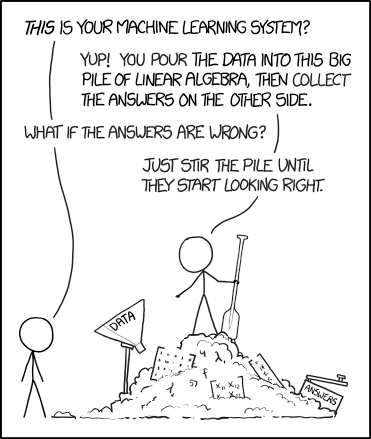
\includegraphics[height=0.55\textheight]{images/1838_machine_learning.png}
\end{center}
\bottomnote{XKCD \#1838 by Randall Munroe (CC BY-NC 2.5)}
\end{frame}

% SLIDE 3: Learning Objectives
\begin{frame}[t]{Learning Objectives}
\vspace{1em}
After this lecture, you will be able to:
\begin{itemize}
  \item \textbf{Interpret} embedding visualizations to assess representation quality
  \item \textbf{Analyze} RL training dynamics through reward and value function charts
  \item \textbf{Compare} exploration strategies using cumulative regret analysis
\end{itemize}
\bottomnote{We cover 20 essential visualizations spanning word embeddings, reinforcement learning, and advanced topics}
\end{frame}

% SLIDE 4: Table of Contents
\begin{frame}{Outline}
  \tableofcontents
\bottomnote{Three parts: Word Embeddings, Reinforcement Learning, Advanced Topics}
\end{frame}

% ============================================================
% PART 1: WORD EMBEDDINGS (7 charts)
% ============================================================
\section{Word Embeddings}

% SLIDE 5: C1 --- Embedding Space (REUSE)
\begin{frame}[t]{Words as Vectors: The Embedding Space}
\begin{center}

\includegraphics[width=0.65\textwidth]{01_word_embedding_space/chart.pdf}
\end{center}
\bottomnote{Words with similar meanings cluster together in the high-dimensional embedding space}
\end{frame}

% SLIDE 6: C2 --- Similarity Heatmap (REUSE)
\begin{frame}[t]{Cosine Similarity Between Word Vectors}
\begin{center}

\includegraphics[width=0.65\textwidth]{02_similarity_heatmap/chart.pdf}
\end{center}
\bottomnote{Cosine similarity measures the angle between word vectors---closer to 1 means more semantically similar}
\end{frame}

% SLIDE 7: C3 --- Skip-gram Architecture (REUSE)
\begin{frame}[t]{How Embeddings Are Learned: Skip-gram}
\begin{center}

\includegraphics[width=0.65\textwidth]{08_skipgram_architecture/chart.pdf}
\end{center}
\bottomnote{Skip-gram predicts context words from a center word, learning useful representations as a byproduct}
\end{frame}

% SLIDE 8: C4 --- Negative Sampling (REUSE)
\begin{frame}[t]{Efficient Training: Negative Sampling}
\begin{center}

\includegraphics[width=0.65\textwidth]{10_negative_sampling/chart.pdf}
\end{center}
\bottomnote{Negative sampling avoids computing the full softmax by contrasting true pairs with random negatives}
\end{frame}

% SLIDE 9: C8 --- Word Analogy (NEW)
\begin{frame}[t]{Word Analogy Arithmetic}
\begin{center}

\includegraphics[width=0.65\textwidth]{top10_08_word_analogy/chart.pdf}
\end{center}
\bottomnote{Vector arithmetic captures semantic relationships: the gender direction is consistent across word pairs}
\end{frame}

% SLIDE 10: C10 --- Embedding Dimensions (NEW)
\begin{frame}[t]{How Many Dimensions Do We Need?}
\begin{center}

\includegraphics[width=0.65\textwidth]{top10_10_embedding_dimensions/chart.pdf}
\end{center}
\bottomnote{Similarity structure is well-preserved beyond 20 dimensions; additional dimensions yield diminishing returns}
\end{frame}

% SLIDE 11: A3 --- Nearest Neighbors (NEW)
\begin{frame}[t]{Finding Similar Words in Embedding Space}
\begin{center}

\includegraphics[width=0.65\textwidth]{top10_13_embedding_neighbors/chart.pdf}
\end{center}
\bottomnote{Nearest-neighbor queries retrieve semantically related words---the foundation of many NLP applications}
\end{frame}

% ============================================================
% TRANSITION
% ============================================================

% SLIDE 12: Transition
\begin{frame}[t]{From Representation to Action}
\vspace{1.5em}
\begin{itemize}
  \item Embeddings capture \highlight{meaning} as geometric structure in vector space
  \item Reinforcement learning captures \highlight{behavior} as policies learned from reward signals
  \item Both use \highlight{learned representations} to generalize beyond training examples
\end{itemize}
\bottomnote{Embeddings encode what words mean; RL learns what actions to take---both are fundamental to modern AI}
\end{frame}

% ============================================================
% PART 2: REINFORCEMENT LEARNING (6 charts)
% ============================================================
\section{Reinforcement Learning}

% SLIDE 13: C5 --- Q-Learning Grid (REUSE)
\begin{frame}[t]{Q-Learning: State Values in a Grid}
\begin{center}

\includegraphics[width=0.58\textwidth]{04_q_learning_grid/chart.pdf}
\end{center}
\bottomnote{Q-values encode the expected future reward for each state-action pair in the environment}
\end{frame}

% SLIDE 14: C6 --- Reward Curves (REUSE)
\begin{frame}[t]{Training Progress: Reward Over Episodes}
\begin{center}

\includegraphics[width=0.65\textwidth]{05_reward_curves/chart.pdf}
\end{center}
\bottomnote{Monitoring episode reward over time reveals whether the agent is learning, plateauing, or diverging}
\end{frame}

% SLIDE 15: C7 --- Policy Viz (REUSE)
\begin{frame}[t]{The Learned Policy: What to Do in Each State}
\begin{center}

\includegraphics[width=0.65\textwidth]{06_policy_viz/chart.pdf}
\end{center}
\bottomnote{A policy maps each state to the best action---visualizing it reveals whether the agent has learned sensible behavior}
\end{frame}

% SLIDE 16: C9 --- Epsilon-Greedy (NEW)
\begin{frame}[t]{Exploration vs Exploitation: The Epsilon Tradeoff}
\begin{center}

\includegraphics[width=0.65\textwidth]{top10_09_epsilon_greedy/chart.pdf}
\end{center}
\bottomnote{Too little exploration (greedy) gets stuck on suboptimal arms; too much exploration wastes reward on bad arms}
\end{frame}

% SLIDE 17: A4 --- Q-Value Convergence (NEW)
\begin{frame}[t]{Q-Values Converging to Optimality}
\begin{center}

\includegraphics[width=0.65\textwidth]{top10_14_qvalue_convergence/chart.pdf}
\end{center}
\bottomnote{With sufficient exploration and a decaying learning rate, Q-values provably converge to optimal values}
\end{frame}

% SLIDE 18: A9 --- Gridworld Trajectory (NEW)
\begin{frame}[t]{Optimal vs Random Paths}
\begin{center}

\includegraphics[width=0.58\textwidth]{top10_19_gridworld_trajectory/chart.pdf}
\end{center}
\bottomnote{After training, the learned policy finds the shortest path while random actions meander through the grid}
\end{frame}

% ============================================================
% PART 3: ADVANCED TOPICS (7 charts)
% ============================================================
\section{Advanced Topics}

% SLIDE 19: A1 --- Zipf's Law (NEW)
\begin{frame}[t]{Zipf's Law: The Distribution of Words}
\begin{center}

\includegraphics[width=0.65\textwidth]{top10_11_word_frequency_rank/chart.pdf}
\end{center}
\bottomnote{Zipf's law explains why embedding models must handle both extremely common and rare words}
\end{frame}

% SLIDE 20: A2 --- Context Window (NEW)
\begin{frame}[t]{Context Window Size and Embedding Quality}
\begin{center}

\includegraphics[width=0.65\textwidth]{top10_12_context_window/chart.pdf}
\end{center}
\bottomnote{Small windows capture syntax; larger windows capture semantics---but too large introduces noise}
\end{frame}

% SLIDE 21: A8 --- Embedding PCA Variance (NEW)
\begin{frame}[t]{Embedding Dimensionality Analysis}
\begin{center}

\includegraphics[width=0.65\textwidth]{top10_18_embedding_pca_variance/chart.pdf}
\end{center}
\bottomnote{A few principal components capture most variance, confirming embeddings have low intrinsic dimensionality}
\end{frame}

% SLIDE 22: A5 --- Q-Table Heatmap (NEW)
\begin{frame}[t]{The Full Q-Table: State-Action Values}
\begin{center}

\includegraphics[width=0.65\textwidth]{top10_15_state_action_heatmap/chart.pdf}
\end{center}
\bottomnote{States near the goal have higher Q-values; the optimal action per state has the highest value in its row}
\end{frame}

% SLIDE 23: A6 --- Bandit Regret (NEW)
\begin{frame}[t]{Comparing Exploration Strategies}
\begin{center}

\includegraphics[width=0.65\textwidth]{top10_16_bandit_regret/chart.pdf}
\end{center}
\bottomnote{UCB achieves sublinear regret by balancing exploration and exploitation using confidence bounds}
\end{frame}

% SLIDE 24: A7 --- TD Learning (NEW)
\begin{frame}[t]{Temporal Difference Learning: Value Convergence}
\begin{center}

\includegraphics[width=0.65\textwidth]{top10_17_td_learning_update/chart.pdf}
\end{center}
\bottomnote{TD(0) bootstraps value estimates from successor states, converging to true values without full episodes}
\end{frame}

% SLIDE 25: A10 --- Reward Shaping (NEW)
\begin{frame}[t]{Reward Shaping: Sparse vs Dense}
\begin{center}

\includegraphics[width=0.65\textwidth]{top10_20_reward_shaping/chart.pdf}
\end{center}
\bottomnote{Shaped rewards provide learning signal throughout the episode, accelerating convergence over sparse rewards}
\end{frame}

% ============================================================
% CLOSING
% ============================================================
\section{Summary}

% SLIDE 26: Summary Checklist
\begin{frame}[t]{20 Charts You Should Know}
\vspace{0.3em}
\begin{columns}[T]
\begin{column}{0.48\textwidth}
\footnotesize
\begin{enumerate}
  \item Embedding Space
  \item Similarity Heatmap
  \item Skip-gram Architecture
  \item Negative Sampling
  \item Word Analogy
  \item Embedding Dimensions
  \item Nearest Neighbors
  \item Zipf's Law
  \item Context Window
  \item Embedding PCA Variance
\end{enumerate}
\end{column}
\begin{column}{0.48\textwidth}
\footnotesize
\begin{enumerate}
  \setcounter{enumi}{10}
  \item Q-Learning Grid
  \item Reward Curves
  \item Policy Visualization
  \item Epsilon-Greedy
  \item Q-Value Convergence
  \item Gridworld Trajectory
  \item Q-Table Heatmap
  \item Bandit Regret
  \item TD Learning
  \item Reward Shaping
\end{enumerate}
\end{column}
\end{columns}
\bottomnote{These 20 visualizations cover embeddings, reinforcement learning foundations, and advanced analysis topics}
\end{frame}

% SLIDE 27: Closing XKCD
\begin{frame}[t]{Until Next Time}
\vspace{0.5em}
\begin{center}
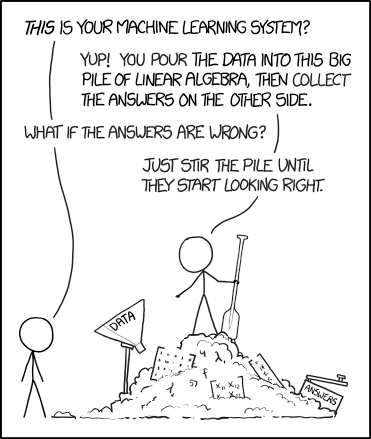
\includegraphics[height=0.55\textheight]{images/1838_machine_learning.png}
\end{center}
\bottomnote{XKCD \#1838 by Randall Munroe (CC BY-NC 2.5)}
\end{frame}

\end{document}
